\section{Простая линейная атака на персептрон}\label{sec:ch1/slap}

Несмотря на широкую практическую применимость нейросетевых моделей, включая многослойный персептрон, их надёжность может быть существенно снижена при воздействии целенаправленных возмущений, известных как состязательные атаки. Эти атаки используют особенности разделяющей поверхности модели для генерации входных данных, вызывающих ошибочную классификацию. В рамках настоящей работы предложен новый подход к формированию таких примеров, получивший название ``простая линейная атака на персептрон`` (SLAP, Simple Linear Attack for Perceptron). Подробности методики опубликованы в авторской статье~\cite{perminov2024slap}.

\nomenclature{MLP}{многослойный персептрон}

%%%%%%%%%%%%%%%%%%%%%%%%%%%%%%%%%%%%%%%%%%%%%%%%%%%%%%%%%%%%%%%%%%%%%%%%%%%%%%%%%%%%%%%%%%%%%%%%%%%%%%%%%%%%%%%
\subsection{Существующие подходы}

Наиболее распространённые методы формирования атакующих примеров основываются на градиентной оптимизации. В частности, метод FGSM (Fast Gradient Sign Method)~\cite{goodfellow2014explaining} и метод проецированного градиентного спуска PGD (Projected Gradient Descent)~\cite{madry2017towards} находят направления в пространстве входных признаков, по которым можно максимизировать ошибку классификатора. Однако такие подходы требуют итеративных вычислений и чувствительны к выбору гиперпараметров.

Альтернативой являются методы, использующие выпуклую оптимизацию или линейное программирование, например,~\cite{croce2019sparse, wong2018provable}. В настоящей работе предложен подход, основанный исключительно на методах линейной алгебры, позволяющий строить атакующие примеры за счёт решения систем линейных уравнений или неравенств. Подход ориентирован прежде всего на персептроны с кусочно-линейными функциями активации, такими как ReLU, Leaky ReLU и Abs, что позволяет упростить структуру модели до линейных преобразований при фиксированных знаках активации.

%%%%%%%%%%%%%%%%%%%%%%%%%%%%%%%%%%%%%%%%%%%%%%%%%%%%%%%%%%%%%%%%%%%%%%%%%%%%%%%%%%%%%%%%%%%%%%%%%%%%%%%%%%%%%%%
\subsection{Постановка задачи атаки}

\fixme{ЗАМЕНИТЬ \(n\) НА \(d\) и \(m\) на \(C\) поправить рисунки}

Пусть имеется обученный персептрон \(c(x)\), принимающий на вход вектор \(x \in \mathbb{R}^d\) и возвращающий вектор выходных значений \(y \in \mathbb{R}^C\), соответствующих \(C\) (\(C < d\)) классам. Обозначим через \(x_t\) целевой пример (рисунок~\cref{fig:attack_task}\subcaptionref{fig:attack_task_x_t}), на который должна быть «перенесена» классификация, и через \(x_a\) -- пример, который подвергается атаке (рисунок~\cref{fig:attack_task}\subcaptionref{fig:attack_task_x_a}). Требуется построить новый вектор \(x\) (рисунок~\cref{fig:attack_task}\subcaptionref{fig:attack_task_x}), близкий к \(x_a\), но классифицируемый так же, как \(x_t\). Формально, задача формулируется как:

\[
\begin{cases}
    \| x - x_a \| \rightarrow \min,\\
    \| x - x_t \| > 0,\\
    c(x) = c(x_t),
\end{cases}
\quad \text{или} \quad
\begin{cases}
    \| x - x_a \| \rightarrow \min,\\
    \| x - x_t \| > 0,\\
    \arg\max c(x) = \arg\max c(x_t).
\end{cases}
\]

\begin{figure}[ht]
    \centerfloat{
        \hfill
        \subcaptionbox{\(x_t\) -- целевой пример\label{fig:attack_task_x_t}}{%
            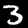
\includegraphics[width=0.3\linewidth]{Dissertation/images/ch1/slap/x_t.png}}
        \hfill
        \subcaptionbox{\(x_a\) -- пример, подвергающийся атаке\label{fig:attack_task_x_a}}{%
            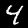
\includegraphics[width=0.3\linewidth]{Dissertation/images/ch1/slap/x_a.png}}
        \hfill
        \subcaptionbox{\(x\) -- построенный атакующий пример\label{fig:attack_task_x}}{%
            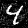
\includegraphics[width=0.3\linewidth]{Dissertation/images/ch1/slap/x.png}}
        \hfill
    }
    \caption{Примеры, участвующие в атаке на многослойный персептрон}
    \label{fig:attack_task}
\end{figure}

Для повышения скрытности атаки накладываются ограничения на диапазон допустимых значений \(x \in [x_{\min}, x_{\max}]\), где, например, для изображений естественно полагать \(x_{\min} = 0\), \(x_{\max} = 1\).

%%%%%%%%%%%%%%%%%%%%%%%%%%%%%%%%%%%%%%%%%%%%%%%%%%%%%%%%%%%%%%%%%%%%%%%%%%%%%%%%%%%%%%%%%%%%%%%%%%%%%%%%%%%%%%%
\subsection{Атака на однослойный персептрон}

Рассмотрим случай одного слоя, где выходной вектор модели задаётся как \(y = Wx + b\), причём \(W \in \mathbb{R}^{C \times d} \), \(b \in \mathbb{R}^C\).

\subsubsection{Без учёта ограничений на входные значения}

Предположим, что матрицу \(W\) можно разбить на подматрицы \(W_1 \in \mathbb{R}^{C \times C}\) и \(W_2 \in \mathbb{R}^{C \times (d - C)}\), выбрав, например, первые (или случайные для большей незаметности) \(C\) столбцов. Аналогично разбиваем вектор \(x_a\) на \(x_{a_1} \in \mathbb{R}^C\) и \(x_{a_2} \in \mathbb{R}^{d - C}\). Тогда атакующий вектор может быть получен по формуле:

\[
x^* = W_1^{-1} \cdot (b^\top - W_2 x_{a_2}),
\]
а полное решение восстанавливается как конкатенация \(x = [x^*, x_{a_2}]\) (рисунок~\cref{fig:matrix_attack}).

\begin{figure}[ht]
    \centerfloat{
        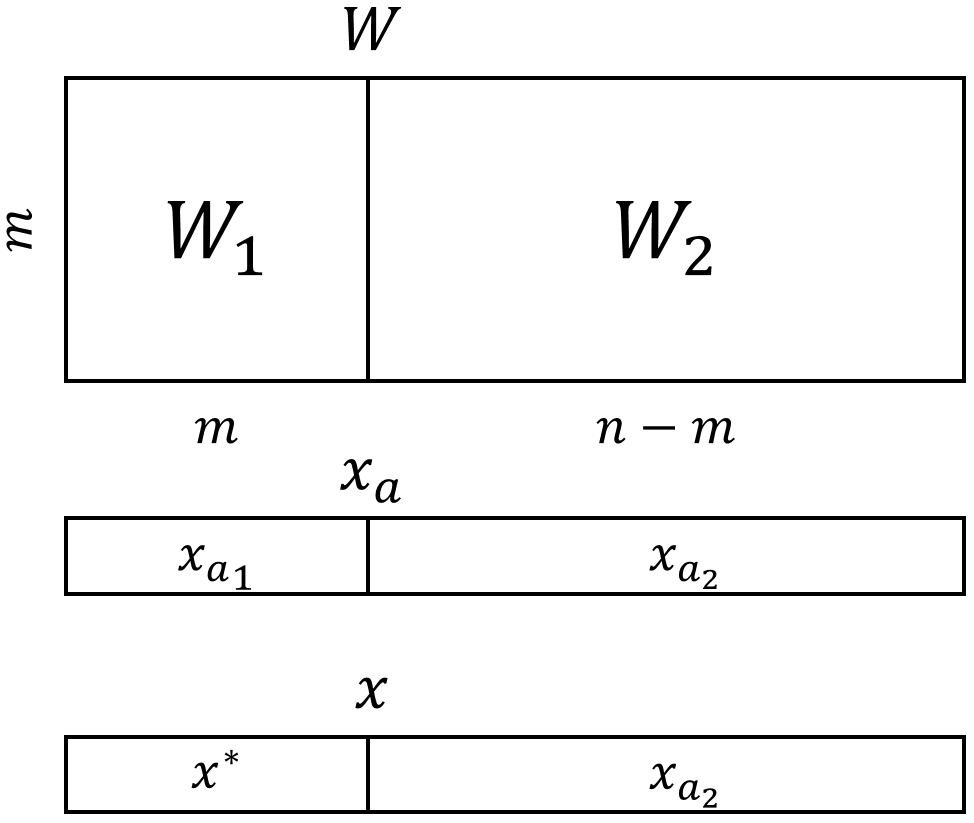
\includegraphics[width=0.7\linewidth]{Dissertation/images/ch1/slap/matrix_attack.png}
    }
    \caption{Схема матричной атаки}
    \label{fig:matrix_attack}
\end{figure}

Данный метод работает исключительно в случае, если матрица \(W_1\) обратима (что почти всегда выполняется при случайной инициализации). Однако он не учитывает допустимые границы значений и чувствителен к квантованию, происходящему при сохранении изображения в файл (рисунок~\cref{fig:matrix_attack_example}).

\begin{figure}[ht]
    \centerfloat{
        \hfill
        \subcaptionbox{\(x_t\) -- целевой пример}{%
            
\includegraphics[width=0.3\linewidth]{Dissertation/images/ch1/slap/matrix_x_t.jpeg}}
        \hfill
        \subcaptionbox{\(x_a\) -- пример, который подвергается атаке}{%
            
\includegraphics[width=0.3\linewidth]{Dissertation/images/ch1/slap/matrix_x_a.jpeg}}
        \hfill
        \subcaptionbox{\(x\) -- построенный атакующий пример}{%
            
\includegraphics[width=0.3\linewidth]{Dissertation/images/ch1/slap/matrix_x.jpeg}}
        \hfill
    }
    \caption{Пример матричной атаки, \(x \in [-1055, 926]\)}
    \label{fig:matrix_attack_example}
\end{figure}

\subsubsection{С учётом ограничений}

Более реалистичный подход включает в себя формулировку задачи как квадратичной оптимизации:

\[
\begin{cases}
    \frac{1}{2} x^\top P x + q^\top x \rightarrow \min,\\
    Ax = b,\\
    x_{\min} \leq x \leq x_{\max},
\end{cases}
\]
где в простейшем случае \(P = E\) -- единичная матрица, \(q = -x_a\), \(A = W\), \(b = y_t - b\). Тогда задача принимает вид:

\[
\begin{cases}
    \frac{1}{2} x^\top x + x_a^\top x \rightarrow \min,\\
    Wx = y_t - b,\\
    x \in [x_{\min}, x_{\max}].
\end{cases}
\]

При невозможности точного воспроизведения \(y_t\) возможно ослабление условий за счёт введения допусков \(\epsilon\):

\[
y_t - \epsilon \leq Wx + b \leq y_t + \varepsilon.
\]

Эти неравенства легко переписываются в канонической форме для QP-решателей. Пример применения данного вида атаки приведён на рисунке~\cref{fig:qp_attack_example}.

\begin{figure}[ht]
    \centerfloat{
        \hfill
        \subcaptionbox{\(x_t\) -- целевой пример}{%
            
\includegraphics[width=0.3\linewidth]{Dissertation/images/ch1/slap/qp_x_t.png}}
        \hfill
        \subcaptionbox{\(x_a\) -- пример, который подвергается атаке}{%
            
\includegraphics[width=0.3\linewidth]{Dissertation/images/ch1/slap/qp_x_a.png}}
        \hfill
        \subcaptionbox{\(x\) -- построенный атакующий пример}{%
            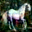
\includegraphics[width=0.3\linewidth]{Dissertation/images/ch1/slap/qp_x.png}}
        \hfill
    }
    \caption{Пример QP атаки}
    \label{fig:qp_attack_example}
\end{figure}

%%%%%%%%%%%%%%%%%%%%%%%%%%%%%%%%%%%%%%%%%%%%%%%%%%%%%%%%%%%%%%%%%%%%%%%%%%%%%%%%%%%%%%%%%%%%%%%%%%%%%%%%%%%%%%%
\subsection{Атака на многослойный персептрон}

При наличии нескольких слоёв в сети возникает проблема нелинейности из-за активационных функций. Однако, если эти функции кусочно-линейны (ReLU, Leaky ReLU, Abs), то при фиксированных знаках аргументов они представляют собой линейные отображения. Например, функция ReLU ведёт себя как \(x\) при \(x \geq 0\) и как \(0\) при \(x < 0\).

Рассмотрим модель из трёх слоёв:

\[
y = W_3 \cdot f_2(W_2 \cdot f_1(W_1 x + b_1) + b_2) + b_3.
\]

Предположим, что знаки активации известны (например, получены от прямого прохода по \(x_t\)). Тогда последовательное раскрытие слоёв позволяет свести сеть к линейной модели. Например, если все значения после первого слоя положительны (т.е. активация \(f_1\) действует как тождественная функция), а после второго -- отрицательны (и активация действует как умножение на константу), можно получить:

\[
\begin{cases}
    W_1x + b_1 \geq 0\\
    W_2W_1x + W_2b_1 + b_2 \leq 0\\
    y = -(W_3W_2W_1x + W_3W_2b_1 + W_3b_2) + b_3 
\end{cases}
\]
где коэффициенты \(W_{321}\), \(b_{321}\) выражаются через произведения матриц весов и сдвигов. Тогда атака сводится к аналогичной задаче QP, но при дополнительных ограничениях на знаки промежуточных переменных:

\[
\begin{cases}
    W_{21} = W_2W_1\\
    b_{21} = W_2b_1 + b_2\\
    W_{321} = -W_3W_2W_1\\
    b_{321} = b_3 - W_3W_2b_1 - W_3b_2\\
    W_1x + b_1 \geq 0\\
    W_{21}x + b_{21} \leq 0\\
    y = W_{321}x + b_{321}
\end{cases}
\]

Пример атаки на многослойный персептрон представлен на рисунке~\cref{fig:multilayer_attack_example}.

\begin{figure}[ht]
    \centerfloat{
        \hfill
        \subcaptionbox{\(x_t\) -- целевой пример}{%
            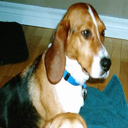
\includegraphics[width=0.3\linewidth]{Dissertation/images/ch1/slap/multilayer_x_t.png}}
        \hfill
        \subcaptionbox{\(x_a\) -- пример, который подвергается атаке}{%
            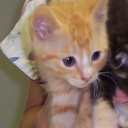
\includegraphics[width=0.3\linewidth]{Dissertation/images/ch1/slap/multilayer_x_a.png}}
        \hfill
        \subcaptionbox{\(x\) -- построенный атакующий пример}{%
            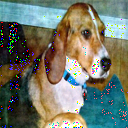
\includegraphics[width=0.3\linewidth]{Dissertation/images/ch1/slap/multilayer_x.png}}
        \hfill
    }
    \caption{Пример атаки на многослойный персептрон на датасете Cat-vs-Dog~\cite{parkhi2012cats}}
    \label{fig:multilayer_attack_example}
\end{figure}

%%%%%%%%%%%%%%%%%%%%%%%%%%%%%%%%%%%%%%%%%%%%%%%%%%%%%%%%%%%%%%%%%%%%%%%%%%%%%%%%%%%%%%%%%%%%%%%%%%%%%%%%%%%%%%%
\subsection{Генерация произвольных входов с заданным выходом}

Так как размерность входа чаще всего превышает размерность выхода, задача построения входа \(x\), удовлетворяющего \(c(x) = y_t\), имеет бесконечно много решений. В этом случае можно случайным образом зафиксировать некоторые координаты \(x\), оставляя другие свободными, и решать полученную переопределённую систему. Это позволяет формировать обширные множества атакующих примеров, обладающих одинаковым выходом сети.

На рисунке~\cref{fig:bonus_attack} приведены примеры атакующих изображений. В первом столбце расположены целевые изображения, соответствующие заданному выходу модели. Второй столбец содержит атакующие примеры, полученные путём минимального возмущения других исходных изображений с целью приведения их к тому же выходу. Остальные столбцы демонстрируют изображения, сгенерированные методом случайного поиска при условии воспроизведения целевого выхода. Все изображения в пределах одной строки имеют идентичный выходной вектор персептрона, несмотря на различия в визуальном представлении.

\begin{figure}[ht]
    \centerfloat{
        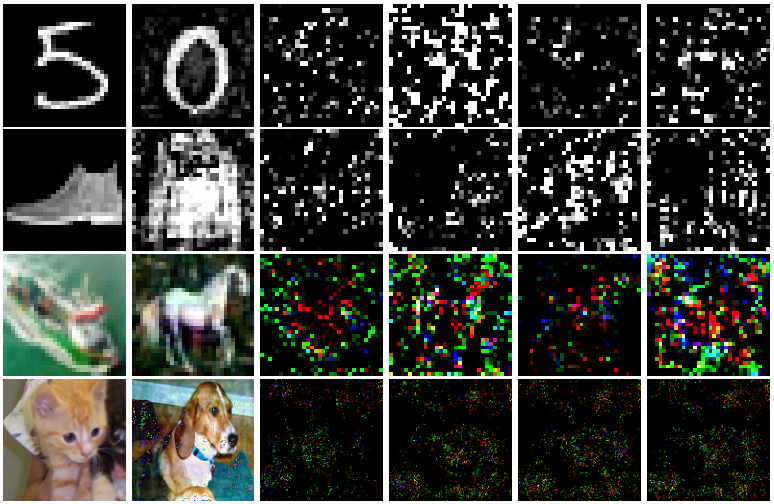
\includegraphics[width=\linewidth]{Dissertation/images/ch1/slap/bonus.png}
    }
    \caption{Пример генерации атакующих примеров}
    \label{fig:bonus_attack}
\end{figure}

%%%%%%%%%%%%%%%%%%%%%%%%%%%%%%%%%%%%%%%%%%%%%%%%%%%%%%%%%%%%%%%%%%%%%%%%%%%%%%%%%%%%%%%%%%%%%%%%%%%%%%%%%%%%%%%
\subsection{Экспериментальное исследование}

Алгоритм был реализован и протестирован на простых персептронах, обученных на датасетах MNIST~\cite{deng2012mnist} и CIFAR-10~\cite{krizhevsky2009learning}. Для каждого изображения из тестовой выборки выбиралось случайное изображение другого класса, и применялась атака, направленная на минимальное изменение первого изображения с целью получения выхода второго. В эксперименте оценивалась \(\ell_\infty\)-норма между оригиналом и атакующим примером. Результаты приведены в таблице~\cref{tab:slap}.

\begin{table} [htbp]
\centering
\begin{threeparttable}
\caption{Результаты применения SLAP атаки}\label{tab:slap}
\begin{SingleSpace}
\begin{tabular}{|l|c|c|c|c|c|c|}
\hline
\multicolumn{1}{|c|}{\multirow{2}{*}{Модель}} &
\multicolumn{1}{|c|}{\multirow{2}{*}{Набор}} &
\multicolumn{1}{|c|}{\multirow{2}{*}{Accuracy}} &
\multicolumn{2}{c|}{Атака на значения} & \multicolumn{2}{c|}{Атака на класс} \\
\cline{4-7}
& & & \(\ell_\infty\) & Accuracy & \(\ell_\infty\) & Accuracy \\
\hline
10               & \multirow{5}{*}{MNIST} & 0.9288 & 0.019 & 0.003 & 0.019 & 0.002 \\
10-10            &                        & 0.9326 & 0.021 & 0.007 & 0.022 & 0.001 \\
100-10           &                        & 0.9805 & 0.052 & 0.009 & 0.051 & 0.005 \\
1000-10          &                        & 0.9849 & 0.091 & 0.012 & 0.092 & 0.009 \\
160-80-40-20-10  &                        & 0.9792 & 0.117 & 0.000 & 0.114 & 0.000 \\
\hline
10               & \multirow{4}{*}{CIFAR10} & 0.3989 & 0.027 & 0.014 & 0.024 & 0.011 \\
100-10           &                          & 0.4853 & 0.054 & 0.032 & 0.055 & 0.018 \\
1000-10          &                          & 0.5236 & 0.095 & 0.041 & 0.096 & 0.023 \\
320-160-80-40-10 &                          & 0.5353 & 0.121 & 0.049 & 0.119 & 0.037 \\
\hline
\end{tabular}
\end{SingleSpace}
\end{threeparttable}
\end{table}

Результаты показывают, что при использовании простых архитектур удаётся достигать атакующих примеров с минимальными отклонениями, зачастую визуально незаметными. При переходе к более глубоким моделям число необходимых изменений возрастает, что объясняется более сложной геометрией границ принятия решений.

%%%%%%%%%%%%%%%%%%%%%%%%%%%%%%%%%%%%%%%%%%%%%%%%%%%%%%%%%%%%%%%%%%%%%%%%%%%%%%%%%%%%%%%%%%%%%%%%%%%%%%%%%%%%%%%
\subsection{Выводы}

Предложенный метод демонстрирует возможность построения состязательных примеров для нейросетевых моделей с кусочно-линейными активациями без использования градиентной информации. Использование методов линейной алгебры позволяет получать как точные, так и приближённые решения с учётом ограничений на значения входных признаков. Атака легко адаптируется к многослойным моделям и может применяться не только к полносвязным сетям, но и к свёрточным архитектурам, обладающим аналогичной линейной структурой.
